\paragraph{Row \& Column counter}
\paragraph{Address counter}
\paragraph{Max \& Min calculator.}

Questo modulo permette di trovare i valori massimo e minimo dei pixel presenti nell'immagine.

Il funzionamento del modulo è semplice. Vengono impiegati due registri: MAX e MIN, nei quali alla fine del calcolo saranno presenti rispettivamente il valore massimo e minimo dei pixel dell'immagine.

Inizialmente,(con l'ausilio del segnale "init") viene caricato nei registri MAX e MIN il valore del primo pixel dell'immagine. Successivamente, per ogni altro pixel dell'immagine, lo si confronta con i valori contenuti nel registro MAX e MIN e, se il valore del pixel è maggiore del massimo (contenuto in MAX) o minore del minimo (contenuto in MIN), si aggiornano i valori nei due registri.

Il calcolo termina dopo aver letto e processato l'ultimo pixel dell'immagine.

\begin{figure}[h!] %%%%     H al posto di h! se dà problemi      %%%%%
  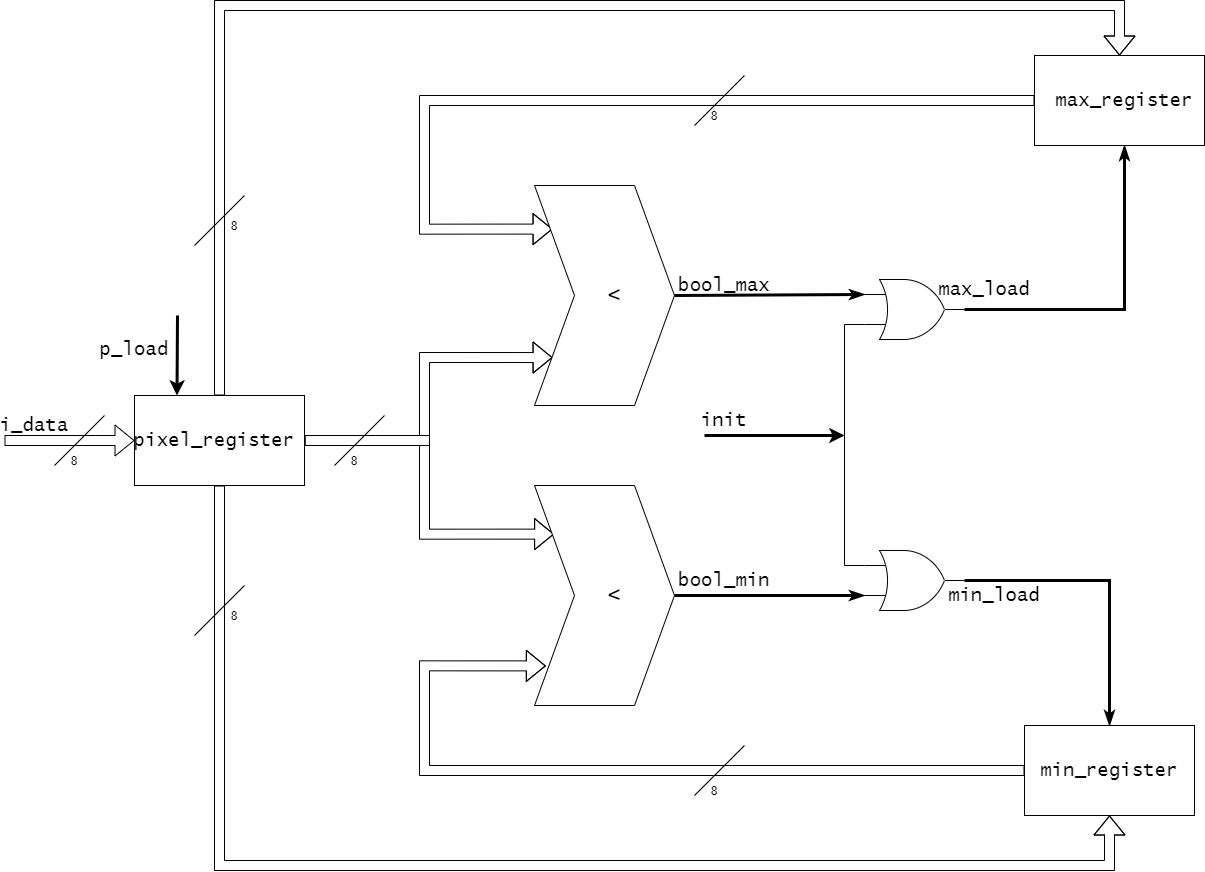
\includegraphics[width=\linewidth]{max_min_module}
  \caption{Max \& Min calculator module.}
  \label{fig:maxMin}
\end{figure}

\paragraph{New pixel value}

Questo modulo è il cuore dell'algoritmo di equalizzazione di immagini, calcola le seguenti funzioni:
\doublespacing
\singlespacing
DELTA\_VALUE = MAX\_PIXEL\_VALUE – MIN\_PIXEL\_VALUE

SHIFT\_LEVEL = (8 – FLOOR(LOG2(DELTA\_VALUE +1)))

TEMP\_PIXEL = (CURRENT\_PIXEL\_VALUE - MIN\_PIXEL\_VALUE) \textless\textless  SHIFT\_LEVEL

NEW\_PIXEL\_VALUE = MIN( 255 , TEMP\_PIXEL)
\doublespacing
\singlespacing
Si presti particolare attenzione al fatto che DELTA\_VALUE assume valori compresi tra 0 e 255, perciò bastano 8 bit per rappresentarlo. Al contrario, DELTA\_VALUE + 1 necessiterà di 9 bit per essere correttamente rappresentato.

L'uscita del logaritmo sarà di 4 bit, poichè i valori da rappresentare sono compresi tra 0 e 8.

La funzione FLOOR(LOG2()) è stata implementata in maniera combinatoria con controlli a soglia:

\begin{table}[h!]
\centering
\begin{tabular}{| c | c |} 
 \hline
 Intervallo & Logaritmo \\
  \hline
 $x \in [~;~]$ & $log_2(x)$ \\ [0.5ex] 
 \hline\hline
 $[1;1]$ & 0 \\ 
 $[2;3]$ & 1 \\
 $[4;7]$ & 2 \\ 
 $[8;15]$ & 3 \\
 $[16;31]$ & 4 \\
 $[32;63]$ & 5 \\
 $[64;127]$ & 6 \\
 $[128;255]$ & 7 \\
 $[256;256]$ & 8 \\ [1ex] 
 \hline
\end{tabular}
\caption{Combinatory logarithm.}
\end{table}

\begin{figure}[h!] %%%%     H al posto di h! se dà problemi      %%%%%
  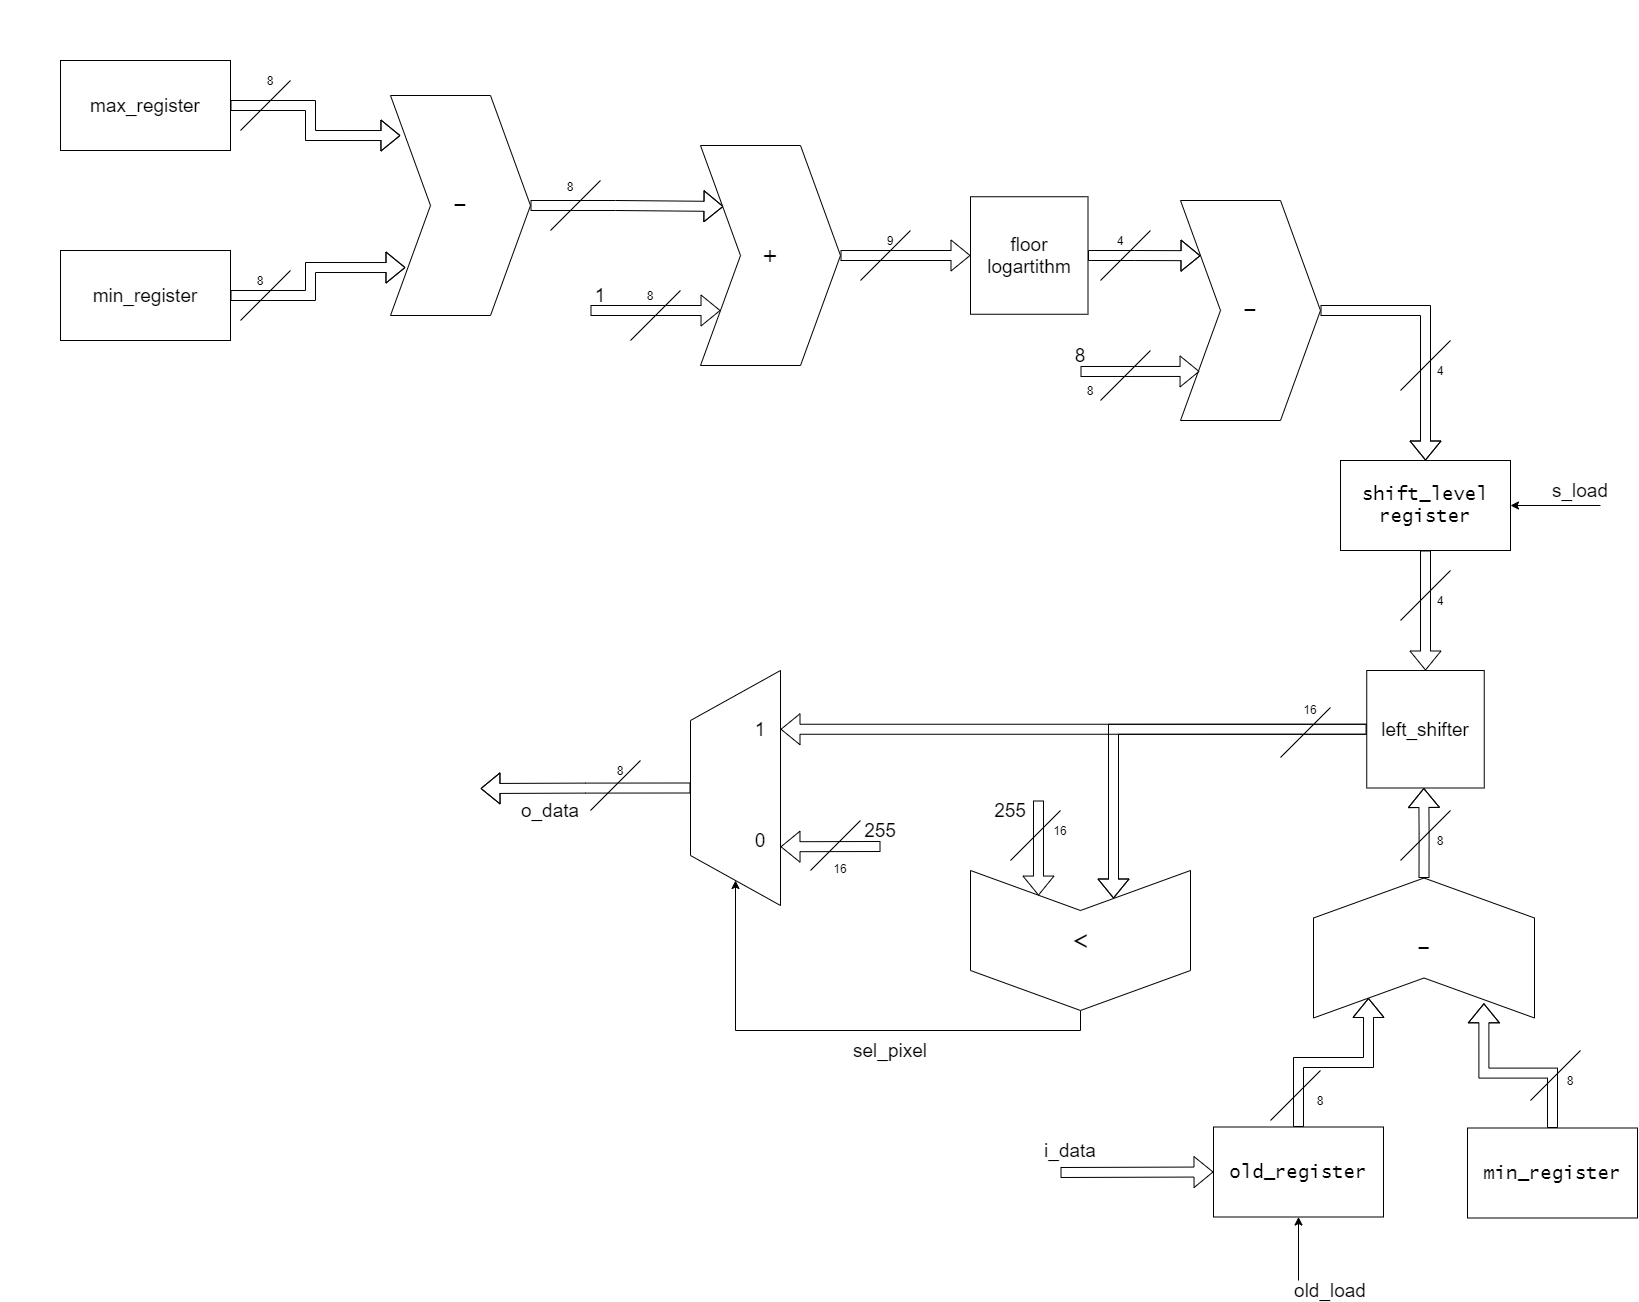
\includegraphics[width=\linewidth]{new_pixel_module}
  \caption{Functions calculator module.}
  \label{fig:newPixel}
\end{figure}
